%% Copernicus Publications Manuscript Preparation Template for LaTeX Submissions
%% ---------------------------------
%% This template should be used for copernicus.cls
%% The class file and some style files are bundled in the Copernicus Latex Package, which can be downloaded from the different journal webpages.
%% For further assistance please contact Copernicus Publications at: production@copernicus.org
%% https://publications.copernicus.org/for_authors/manuscript_preparation.html

%% copernicus_rticles_template (flag for rticles template detection - do not remove!)

%% Please use the following documentclass and journal abbreviations for discussion papers and final revised papers.

%% 2-column papers and discussion papers
\documentclass[gc, manuscript]{copernicus}



%% Journal abbreviations (please use the same for preprints and final revised papers)

% Advances in Geosciences (adgeo)
% Advances in Radio Science (ars)
% Advances in Science and Research (asr)
% Advances in Statistical Climatology, Meteorology and Oceanography (ascmo)
% Annales Geophysicae (angeo)
% Archives Animal Breeding (aab)
% Atmospheric Chemistry and Physics (acp)
% Atmospheric Measurement Techniques (amt)
% Biogeosciences (bg)
% Climate of the Past (cp)
% DEUQUA Special Publications (deuquasp)
% Drinking Water Engineering and Science (dwes)
% Earth Surface Dynamics (esurf)
% Earth System Dynamics (esd)
% Earth System Science Data (essd)
% E&G Quaternary Science Journal (egqsj)
% EGUsphere (egusphere) | This is only for EGUsphere preprints submitted without relation to an EGU journal.
% European Journal of Mineralogy (ejm)
% Fossil Record (fr)
% Geochronology (gchron)
% Geographica Helvetica (gh)
% Geoscience Communication (gc)
% Geoscientific Instrumentation, Methods and Data Systems (gi)
% Geoscientific Model Development (gmd)
% History of Geo- and Space Sciences (hgss)
% Hydrology and Earth System Sciences (hess)
% Journal of Bone and Joint Infection (jbji)
% Journal of Micropalaeontology (jm)
% Journal of Sensors and Sensor Systems (jsss)
% Magnetic Resonance (mr)
% Mechanical Sciences (ms)
% Natural Hazards and Earth System Sciences (nhess)
% Nonlinear Processes in Geophysics (npg)
% Ocean Science (os)
% Polarforschung - Journal of the German Society for Polar Research (polf)
% Primate Biology (pb)
% Proceedings of the International Association of Hydrological Sciences (piahs)
% Safety of Nuclear Waste Disposal (sand)
% Scientific Drilling (sd)
% SOIL (soil)
% Solid Earth (se)
% The Cryosphere (tc)
% Weather and Climate Dynamics (wcd)
% Web Ecology (we)
% Wind Energy Science (wes)

% Pandoc citation processing

% The "Technical instructions for LaTex" by Copernicus require _not_ to insert any additional packages.
% 
% tightlist command for lists without linebreak
\providecommand{\tightlist}{%
  \setlength{\itemsep}{0pt}\setlength{\parskip}{0pt}}


%
\begin{document}


\title{New insights into the Weddell Sea ecosystem applying a network
approach}


\Author[1, *]{Tomás I.}{Marina}
\Author[1, *]{Leonardo A.}{Saravia}
\Author[2]{Susanne}{Kortsch}


\affil[1]{Centro Austral de Investigaciones Científicas (CADIC-CONICET),
Ushuaia, Argentina}
\affil[2]{University of Helsinki, Helsinki, Finland}
\affil[*]{These authors contributed equally to this work.}

\runningtitle{New insights into the Weddell Sea food web}

\runningauthor{Marina et al.}

\correspondence{Tomás I. Marina (tomasimarina@gmail.com) and Leonardo A.
Saravia (arysar@gmail.com)}


\received{}
\pubdiscuss{} %% only important for two-stage journals
\revised{}
\accepted{}
\published{}

%% These dates will be inserted by Copernicus Publications during the typesetting process.


\firstpage{1}

\maketitle


\begin{abstract}
Network approaches can shed light on the structure and stability of
complex marine communities. In recent years, such approaches have been
successfully applied to study polar ecosystems, improving our knowledge
on how they might respond to ongoing environmental changes. The Weddell
Sea is one of the most studied marine ecosystems outside the Antarctic
Peninsula in the Southern Ocean. Yet, few studies consider the known
complexity of the Weddell Sea food web which in its current form
comprises 490 species and 16041 predator-prey interactions. Here we
analysed the Weddell Sea food web, focusing on trophic interactions that
underpin ecosystem structure and stability. We estimated the strength
for each interaction in the food web, characterised species position in
the food web using unweighted and weighted properties, and analysed
species' roles with respect to the stability of the food web. On one
hand, we found that the distribution of the interaction strength at the
food web level is asymmetric, where weak interactions are prevalent.
Including such information as a (weighted) property for species we
detected a positive relationship between species mean interaction
strength and two unweighted properties, trophic level and the total
number of interactions. We also found that only a few species are key in
terms of food web stability, presenting high mean interaction strength,
mid to high trophic level, relatively high number of interactions, and
mid to low trophic similarity. In the same analysis we have integrated
food web and species information, enabling a more complete assessment of
the ecosystem structure and function, likely highlighting the ecological
processes at play in the Weddell Sea. We consider that our results
provide new insights important for the development of effective policies
and management strategies, particularly given the ongoing initiative to
implement a Marine Protected Area (MPA) in the Weddell Sea.
\end{abstract}




\section{Introduction}

Building a network of feeding interactions among species is a
fundamental step to understand ecological communities and is a valuable
tool to manage ecosystems for conservation of biodiversity and
functioning \citep{Thompson2012}. Although analyses considering
presence/absence data on predator-prey interactions have provided
insights about the structure and functioning of communities
\citep[e.g.][]{Kortsch2015, Marina2018, Cordone2020, Rodriguez2022},
more information is needed to effectively charaterise the ecosystems'
dynamics and stability. In this regard, the intensity of the
interactions between species or the interaction strength became of
paramount importance in recent years
\citep{Carrara2015, Allesina2015, Nilsson2016}.

Several methodologies have been applyied to estimate the interaction
strength in food webs, where the quantity and quality of data mostly
determines which approach is more convenient \citep{Berlow2004}.

The Weddell Sea represents the southerly part of the Atlantic Sector of
the Southern Ocean. About one quarter of the Weddell Sea's entire marine
area lies over the continental shelf, stretching along the eastern
contour of the Antarctic Peninsula and the Antarctic continent up to
20◦E. The ecosystem of the Weddell Sea is one of the most pristine and
relatively unexplored hotspots of marine biodiversity in Antarctica
\citep{Teschke2021}. It contains several areas of ecological
significance for birds and marine mammals, such as important breeding
and foraging areas \citep{Hindell2020}. Furthermore, the sea floor is
home to large and unique forest-like sponge and filter-feeder
assemblages, which are particularly numerous on the continental shelf in
the eastern part of the Weddell Sea. These species assemblages create a
structurally complex and diverse habitat for thousands of species
{[}\citet{Barthel1992}; \citet{Brey1994}; Brandt2007{]}.

The Weddell Sea region is less affected by sea surface warming compared
with other areas of the Southern Ocean. If a climate change scenario is
considered, the Weddell Sea continental shelf will be probably a sink
area and a refuge for highly cold-adapted benthonic species
\citep{Griffiths2017}.

The objective of this work was to improve the knowledge on how the
Weddell Sea and the species therein may respond to perturbations from
ongoing environmental changes. To achieve this we: 1) estimated the
strength for each interaction in the Weddell Sea food web, 2)
characterised species considering weighted and unweighted properties,
and 3) analysed the species' role in the stability of the food web.

\section{Methodology}

\subsection{Study area}

The high Antarctic Weddell Sea shelf is situated between 74 and 78ºS
stretching approximately 450 km from East to West (Figure 1). Water
depth varies between 200 and 500 meters, and shallower areas are covered
by continental ice, which forms the coastline along the eastern and
southern part of the Weddell Sea. The shelf area contains a complex
benthic three-dimensional habitat with large benthic biomasses,
intermediate to high diversity in comparison to benthic boreal
communities and a spatially patchy distribution of organisms
\citep{Dayton1990, Teixido2002}.

\subsection{Weddell Sea food web dataset}

The Weddell Sea food web was retrieved from the GlobAL daTabasE of
traits and food Web Architecture (GATEWAy, version 1.0) of the German
Centre for Integrative Biodiversity Research (iDiv) Halle-Jena-Leipzig
\citep{Brose2018}. In addition to predator-prey interactions, the
database contains information on other biological data such as the mean
body mass and movement type for each species in the food web.
Furthermore, it incorporates information about the interaction itself,
such as the dimension of the predator search space (2 or 3 dimensions).
In its current form the Weddell Sea food web comprises 490 species and
16041 predator-prey interactions and constitutes one of the most
resolved food webs constructed to date \citep{Jacob2011}.

\subsection{Dataset analyses}

\subsubsection{Interaction strength estimation and distribution}

To estimate the strength of each pairwise interaction in the food web we
followed the methodology proposed by \citet{Pawar2012}. The minimum data
requirements are body mass of the consumer (predator) and resource
(prey), and the interaction dimensionality (ID) classified as 2 or 3
dimensions. The ID is defined as the dimension of the search space of
the predator, that is equivalent to the movement space of the prey.
Thus, the ID is classified as 2D when both predator and prey move in 2D
(e.g., both are benthic) or if a predator moves in 3D and a prey in 2D
(e.g., pelagic predator on benthic prey). The ID is classified as 3D
when both predator and prey move in 3D (e.g., both pelagic) or if the
predator moves in 2D and the prey in 3D (e.g., benthic predator, pelagic
prey) \citep{Pawar2012}. GATEWAy v.1.0 provides information on the mean
body mass for consumers and resources, except for `detritus' and
`sediment', and the dimensionality for the majority of the interactions,
though the latter is missing in some cases (924 interactions). To
complete the missing data on species `dimensionality', we used
information about the movement type of predators and prey included in
GATEWAy.

The main equation we used for estimating the interaction strength IS
was:

\begin{equation}
IS = \alpha x_R \frac{m_R}{m_C}
\end{equation}

where \vec{\alpha} is the search rate, \vec{x_R} is the resource
density, and \vec{m_R} and \vec{m_C} are the body mass for the resource
and the consumer, respectively \citep{Pawar2012}.

We obtained estimates for resource density and the search rate from the
scaling relationships with the resource and the consumer mass,
respectively \citep{Pawar2012}. The coefficients of such relationships,
determined by ordinary least squares regression, vary with the
interaction dimensionality. On one hand, resource density scales with
resource mass as power-law with exponents in 2D and in 3D. Since mean
mass for resources `phytodetritus' and `sediment' were not available in
GATEWAy, we considered the body mass of the smallest phytoplankton
species (`Fragilariopsis cylindrus') as a proxy. This is justified by
the fact that `phytodetritus' and `sediment' are mainly composed of dead
or senescent phytoplankton reaching the seabed \citep{Wolanski2011}. On
the other hand, search rate scales with consumer mass as power-law with
exponents in 2D and in 3D.

We fitted six candidate models (Exponential, Gamma, log-Normal, Normal,
Power-law and Uniform) the interaction strength distribution using
maximum likelihood \citep{McCallum2008}, and selected the best fitting
model by computing the Akaike Information Criterion AIC
\citep{Burnham2002}.

\subsubsection{Species properties}

To characterise the role of each species in the food web, we considered
unweighted and weighted food web properties (Figure 2). Unweighted
properties are related to properties commonly used in qualitative food
web studies and only describe the presence or absence of interactions
without any information on strength between a pairwise species link
\citep{Martinez1991, Dunne2002, Borrelli2014}. In contrast, weighted
properties capture the importance of interaction strength.

To assess species roles as a function of the weighted food web, we
focused on mean interaction strength defined as the average strength of
all interactions for a given species. Further we calculated three
unweighted species properties: a) species degree, i.e., the sum of in-
and out-going interactions ; b) trophic level ; and c) trophic
similarity, i.e., the trophic overlap based on shared and unique
resources and consumers. These metrics were chosen to assess a species
role based on the unweighted food web. The species degree has often been
equated with species importance to the structure and functioning within
a food web, i.e.~perturbations to high-degree species may therefore have
more significant effects on the food web robustness to perturbations
than low-degree species
\citetext{\citealp{Dunne2002a}; \citealp[references
in][]{Cirtwill2018a}}. The trophic level offers information about how
important a species is to its biotic community, i.e., top predators and
primary producers are expected to have particularly large effects on the
rest of their communities through top-down and bottom-up control,
respectively \citep[references in][]{Cirtwill2018a}. Trophic similarity
is an index of trophic overlap considering the set of prey and predators
for a pair of species; it measures one of the most important aspects of
species' niches, the trophic niche, and functional aspects of
biodiversity \citep{Martinez1991, Williams2000}.

Furthermore, we took a species' habitat into account, which describes
the physical position of a species within the ecosystem. Species were
categorised as: 1) benthic, if a species lives on the seafloor; 2)
pelagic, if a species lives close to the surface; 3) benthopelagic, if
it moves between and connects the mentioned environments; 4) demersal,
if it lives and feeds on or near the bottom of the sea; and 5)
land-based, if the consumer is not strictly aquatic but feeds
predominantly on marine species. Species habitat affiliation was
retrieved from \citet{Jacob2011}.

With the aim of studying the relationship between the interaction
strength of the species (weighted property) and its unweighted
properties we performed linear regression analyses between the log mean
interaction strength and each of the mentioned unweighted properties.
Thus we considered the interaction strength as the dependent variable
and the given unweighted property as the independent variable, and
obtained the coefficients (slope and intercept) for the linear model.
Models were fitted using the least squares approach. We also explored
the mean interaction strength distribution with the species habitat.

Formulas used to obtain the above species properties are described in
Supplementary Material.

\subsubsection{Extinction simulations and stability}

To analyse the impact of species on food web stability, we performed
extinction simulations deleting one species at a time, that is for every
extinction network size was reduced by one species only. After each
extinction, we calculated the stability of the network minus the
targeted species (489 nodes) and compared it with that of the whole
network (490 nodes in total). To calculate stability, we used the mean
of the real part of the maximum eigenvalue of the Jacobian matrix using
randomized Jacobians and keeping the predator-prey sign structure fixed
\citep{Allesina2008, Grilli2016}. This index indicates a more stable
food web when it is negative. We performed 1000 simulations for each
species extinction and obtained a mean maximum eigenvalue for each case.
At last we statistically analysed such a difference with an
Anderson-Darling test considering a p-value \textless{} 0.01
\citep{Scholz1987}. If this difference is positive, then the stability
of the food web is higher if a species was removed, and vice versa. A
detailed description on the stability calculations can be found in
Supplementary Material.

Once we had the results for the impact on stability for each species
extinction, we plotted them considering weighted (interaction strength)
and unweighted properties, and species habitat. With this we aim to
characterise those species with a relatively high effect on the
stability of the food web.

All analyses were performed in R software, using the R packages igraph
\citep{Csardi2005}, cheddar \citep{Hudson2013}, and multiweb
\citep{Saravia2019}. The source code and data are available at
https://github.com/EcoComplex/WeddellSea.

\section{Results}

\subsection{Interaction strength distribution}

The statistical distribution that best fitted the empirical interaction
strength distribution of the Weddell Sea food web was a `gamma' due to
the high proportion of weak interactions and the existence of a few
strong interactions (Figure 3, Table S3).

\subsection{Species' role related to their mean interaction strength}

We found that the species' mean interaction strength (weighted property)
shows different relationships with the unweighted properties analysed
(Figure 4A-D). In this regard, there is a positive relationship between
interaction strength and trophic level, i.e., the higher the trophic
level of the species, the higher its mean interaction strength. We also
found a significant but less evident positive relationship with species
degree. Contrary, there was no significant relationship between mean
interaction strength and trophic similarity. Considering species habitat
affiliation, the ``Benthopelagic'' and ``Pelagic'' categories contained
the two species with the highest mean interaction strength, the killer
whale Orcinus orca and the colossal squid Mesonychoteuthis hamiltoni,
respectively. However, the majority of the species with relatively
higher interaction strength belonged to the ``Demersal'' and
``Land-based'' habitats groups. Species inhabiting the benthic realm
showed the lowest mean interaction strength (Figure 4D).

\subsection{Species impact on food web stability}

Our extinction analyses showed that the majority of species had no
significant impact on food web stability after being removed (Figure 5).
Most of the species (black points in figure 5) did not change the
stability of the network considerably after being removed, except for a
few species. Only 15 out of 490 species (3.06\%) gave rise to
significant changes in the food web's stability after their removal
(Table 2). Most of these species had a positive impact on food web
stability, i.e., network stability increased after their removal. Only
two species significantly decreased network stability after being
removed, the demersal fish Pagetopsis macropterus and the benthopelagic
amphipod Maxilliphimedia longipes.

After exploring the stability difference against the species properties
(Figure 5), we found that those species that generated a significant
impact on the stability of the food web were characterised by: 1) high
mean interaction strength; 2) mid to high trophic levels (TL
\textgreater{} 3.2); 3) relatively high number of interactions (Degree
\textgreater{} 25); and 4) mid to low trophic similarity (TS \textless{}
0.16). Habitat wise, species with a significant impact on the stability
were present in all habitats, except for the benthic realm. Table 2
shows these results for such species.

\section{Discussion}

\subsection{Many weak and a few strong interactions}

Our analyses show that the distribution of species interaction strength
at the network level is asymmetric, i.e., the Weddell Sea food web
contains many weak interactions and only a few strong ones. This finding
is consistent with many previous theoretical and empirical studies
\citep[e.g.][]{McCann1998, Neutel2002, Emmerson2004, Wootton2005, Kortsch2021}.
The asymmetric distribution of interaction strength in food webs has
been interpreted as an explanation for the persistence of complex
communities in nature \citep{Bascompte2005, Allesina2015, Nilsson2016}.
Here we show that this pattern is also prevalent in one of the most
complex empirical (marine) food webs to date, comprising 490 species and
16041 predator-prey interactions. This finding reinforces the call for
the inclusion of interaction strength in food web studies to better
understand the ecosystem functioning, and species and whole network
responses to environmental perturbations.

\subsection{Species's role related to their mean interaction strength}

We employed a range of descriptors using both unweighted and weighted
food web properties to characterise the dynamic and multifaceted nature
of the Weddell Sea food web. Our results show a positive relationship
between interaction strength and trophic level, and between interaction
strength and species degree. Mean interaction strength increases with
trophic level and species degree. The former relationship might
contradict those studies that suggest that mid-trophic level species are
involved in the major pathways of energy flow in high-latitude marine
ecosystems
\citep{Pinkerton2014, Murphy2016, McCormack2020, Riccialdelli2020}. This
could be explained by the lack of species biomass data in our
interaction strength estimations; the methodology we applied here
\citep{Pawar2012} allows empirical data for the density of the resource
to be included, though this data is not for the majority of food web
species at the study site. On the other hand, the positive relationship
between interaction strength and degree reinforces the importance of
species with many interactions: species with high degree (hubs) have a
large impact on overall food web structure and functioning
\citep{Dunne2002a, Kortsch2015}. In the Weddell Sea, species with high
degree also tend to have high mean interaction strengths. This
information on the quantity and quality of interactions and its
relationship enables a robust assessment of the species' role in the
stability of the food web \citep{Cirtwill2018a}.

\subsection{Species impact on food web stability}

Only a few species play a key role with respect to the Weddell Sea food
web stability, according to the mean maximum eingenvalue stability index
employed in this study. This is in concordance with other studies on
complex empirical food webs in marine ecosystems in the Arctic and other
locations in Antarctica \citep{Kortsch2015, Marina2018, Rodriguez2022}.
These key species are characterised by a particular set of food web
properties: high to mean interaction strength; mid to high trophic
level; relatively high number of interactions; and mid to low trophic
similarity. In a previous study on sequential extinction simulations for
the Weddell Sea food web, it was found that larger bodied-sized species
could be lost without causing a collapse of the network. A major caveat
of this finding, also recognised by the authors, was that population
dynamics were ignored and hence no top-down extinctions, or other
indirect effects, could occur. In our study we considered such top-down
effects by including information on the species interaction strength,
which is of paramount importance when analysing the response of
perturbations in ecological communities
\citep{McCann1998, Montoya2009, Novak2011}. Thus, our study suggests
that species with high mean interaction strength and high trophic level
need to be considered with particular attention when trying to predict
the effects of perturbations on the Weddell Sea ecosystem. This
conclusion is further reinforced by the finding that these species have
mid to low trophic similarity, which means that few other species of the
food web can occupy the same trophic role. In a review, it was
emphasised that polar pelagic communities are particularly sensitive to
changes due to a low functional redundancy at key trophic levels
\citep{Murphy2016}. Here we provide broader analyses of species impact
on food web robustness by including species from all habitats (benthic,
pelagic and land-based). This suggests that the sensitivity of marine
polar ecosystems to environmental perturbations is a concern also beyond
the pelagic realm.

\clearpage
\conclusions[Conclusions]

Our study goes beyond the current understanding of how species influence
ecosystem structure and stability in the Weddell Sea in particular and
in most polar regions in general \citep{Murphy2016, McCormack2021}. In
the same analysis we have integrated information about weighted
(interaction strength) and unweighted species properties, enabling a
more complete assessment of the species' role in the food web structure
and function, likely highlighting the ecological processes at play in
the Weddell Sea ecosystem.

We consider that the information provided in this study is important for
the development of effective policies and management strategies,
particularly given the ongoing initiative to implement a Marine
Protected Area (MPA) in the Weddell Sea \citep{Teschke2021}.

\clearpage

\begin{figure}
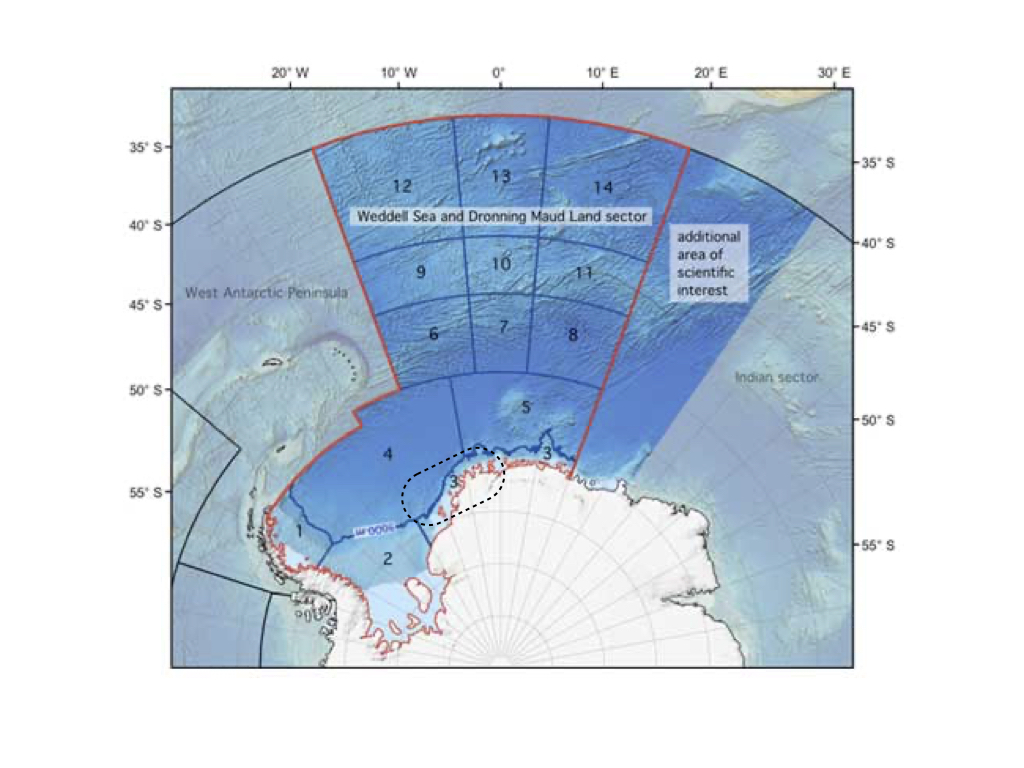
\includegraphics[width=12cm]{Fig.1_StudyMap} \caption{Map of the Weddell Sea and Dronning Maud Land sector highlighting the high Antarctic shelf as a dashed-line contour. Modified from www.soos.aq.}\label{fig:unnamed-chunk-1}
\end{figure}

\clearpage

\begin{figure}
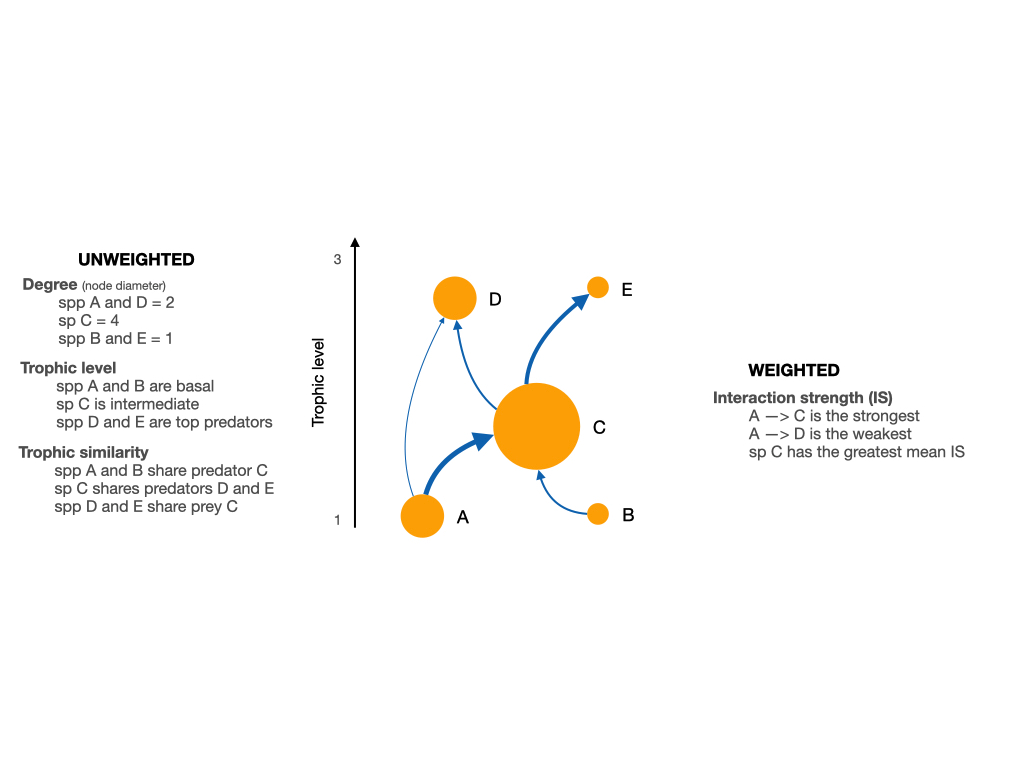
\includegraphics[width=12cm]{Fig.2_ToyFoodWeb} \caption{Scheme of a network showing the weighted and unweighted properties we used to characterize the species of the Weddell Sea food web.}\label{fig:unnamed-chunk-2}
\end{figure}

\clearpage

\begin{figure}
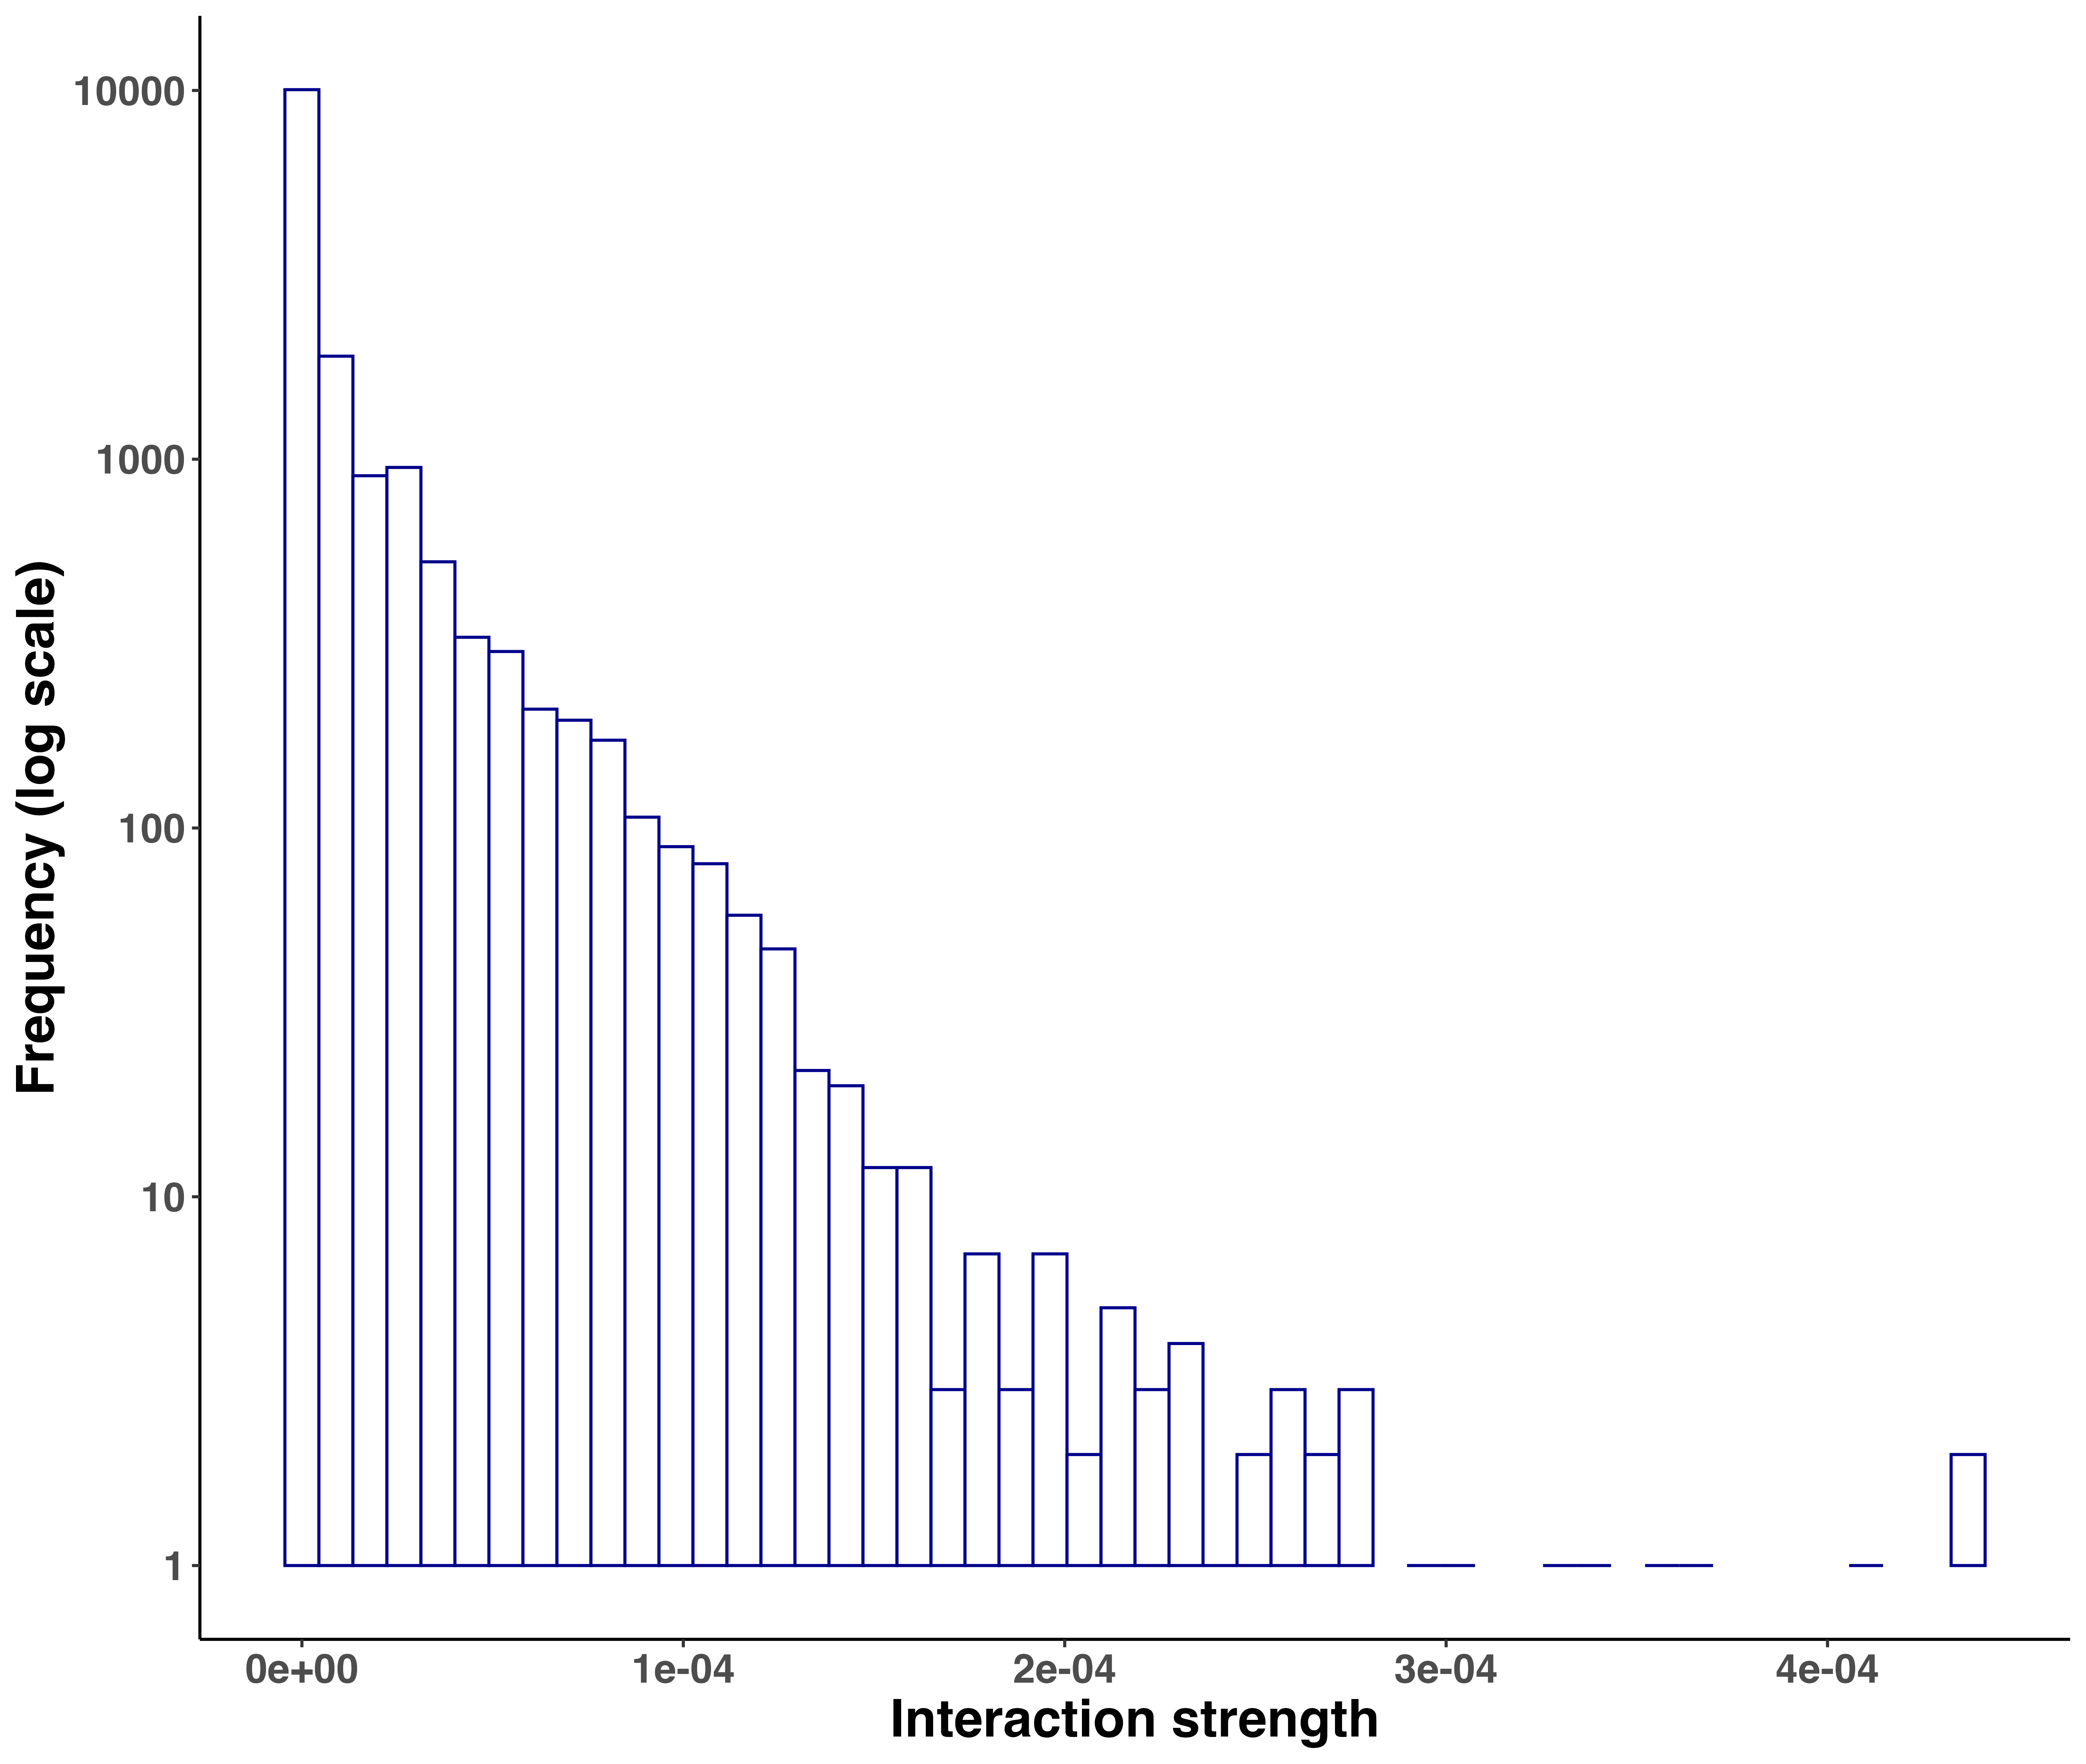
\includegraphics[width=12cm]{Fig3_IntDist} \caption{Frequency distribution of interaction strengths for the Weddell Sea food web. Total number of interactions = 16041. The distribution was best fitted to a ‘gamma’ model.}\label{fig:unnamed-chunk-3}
\end{figure}

\clearpage

\begin{figure}
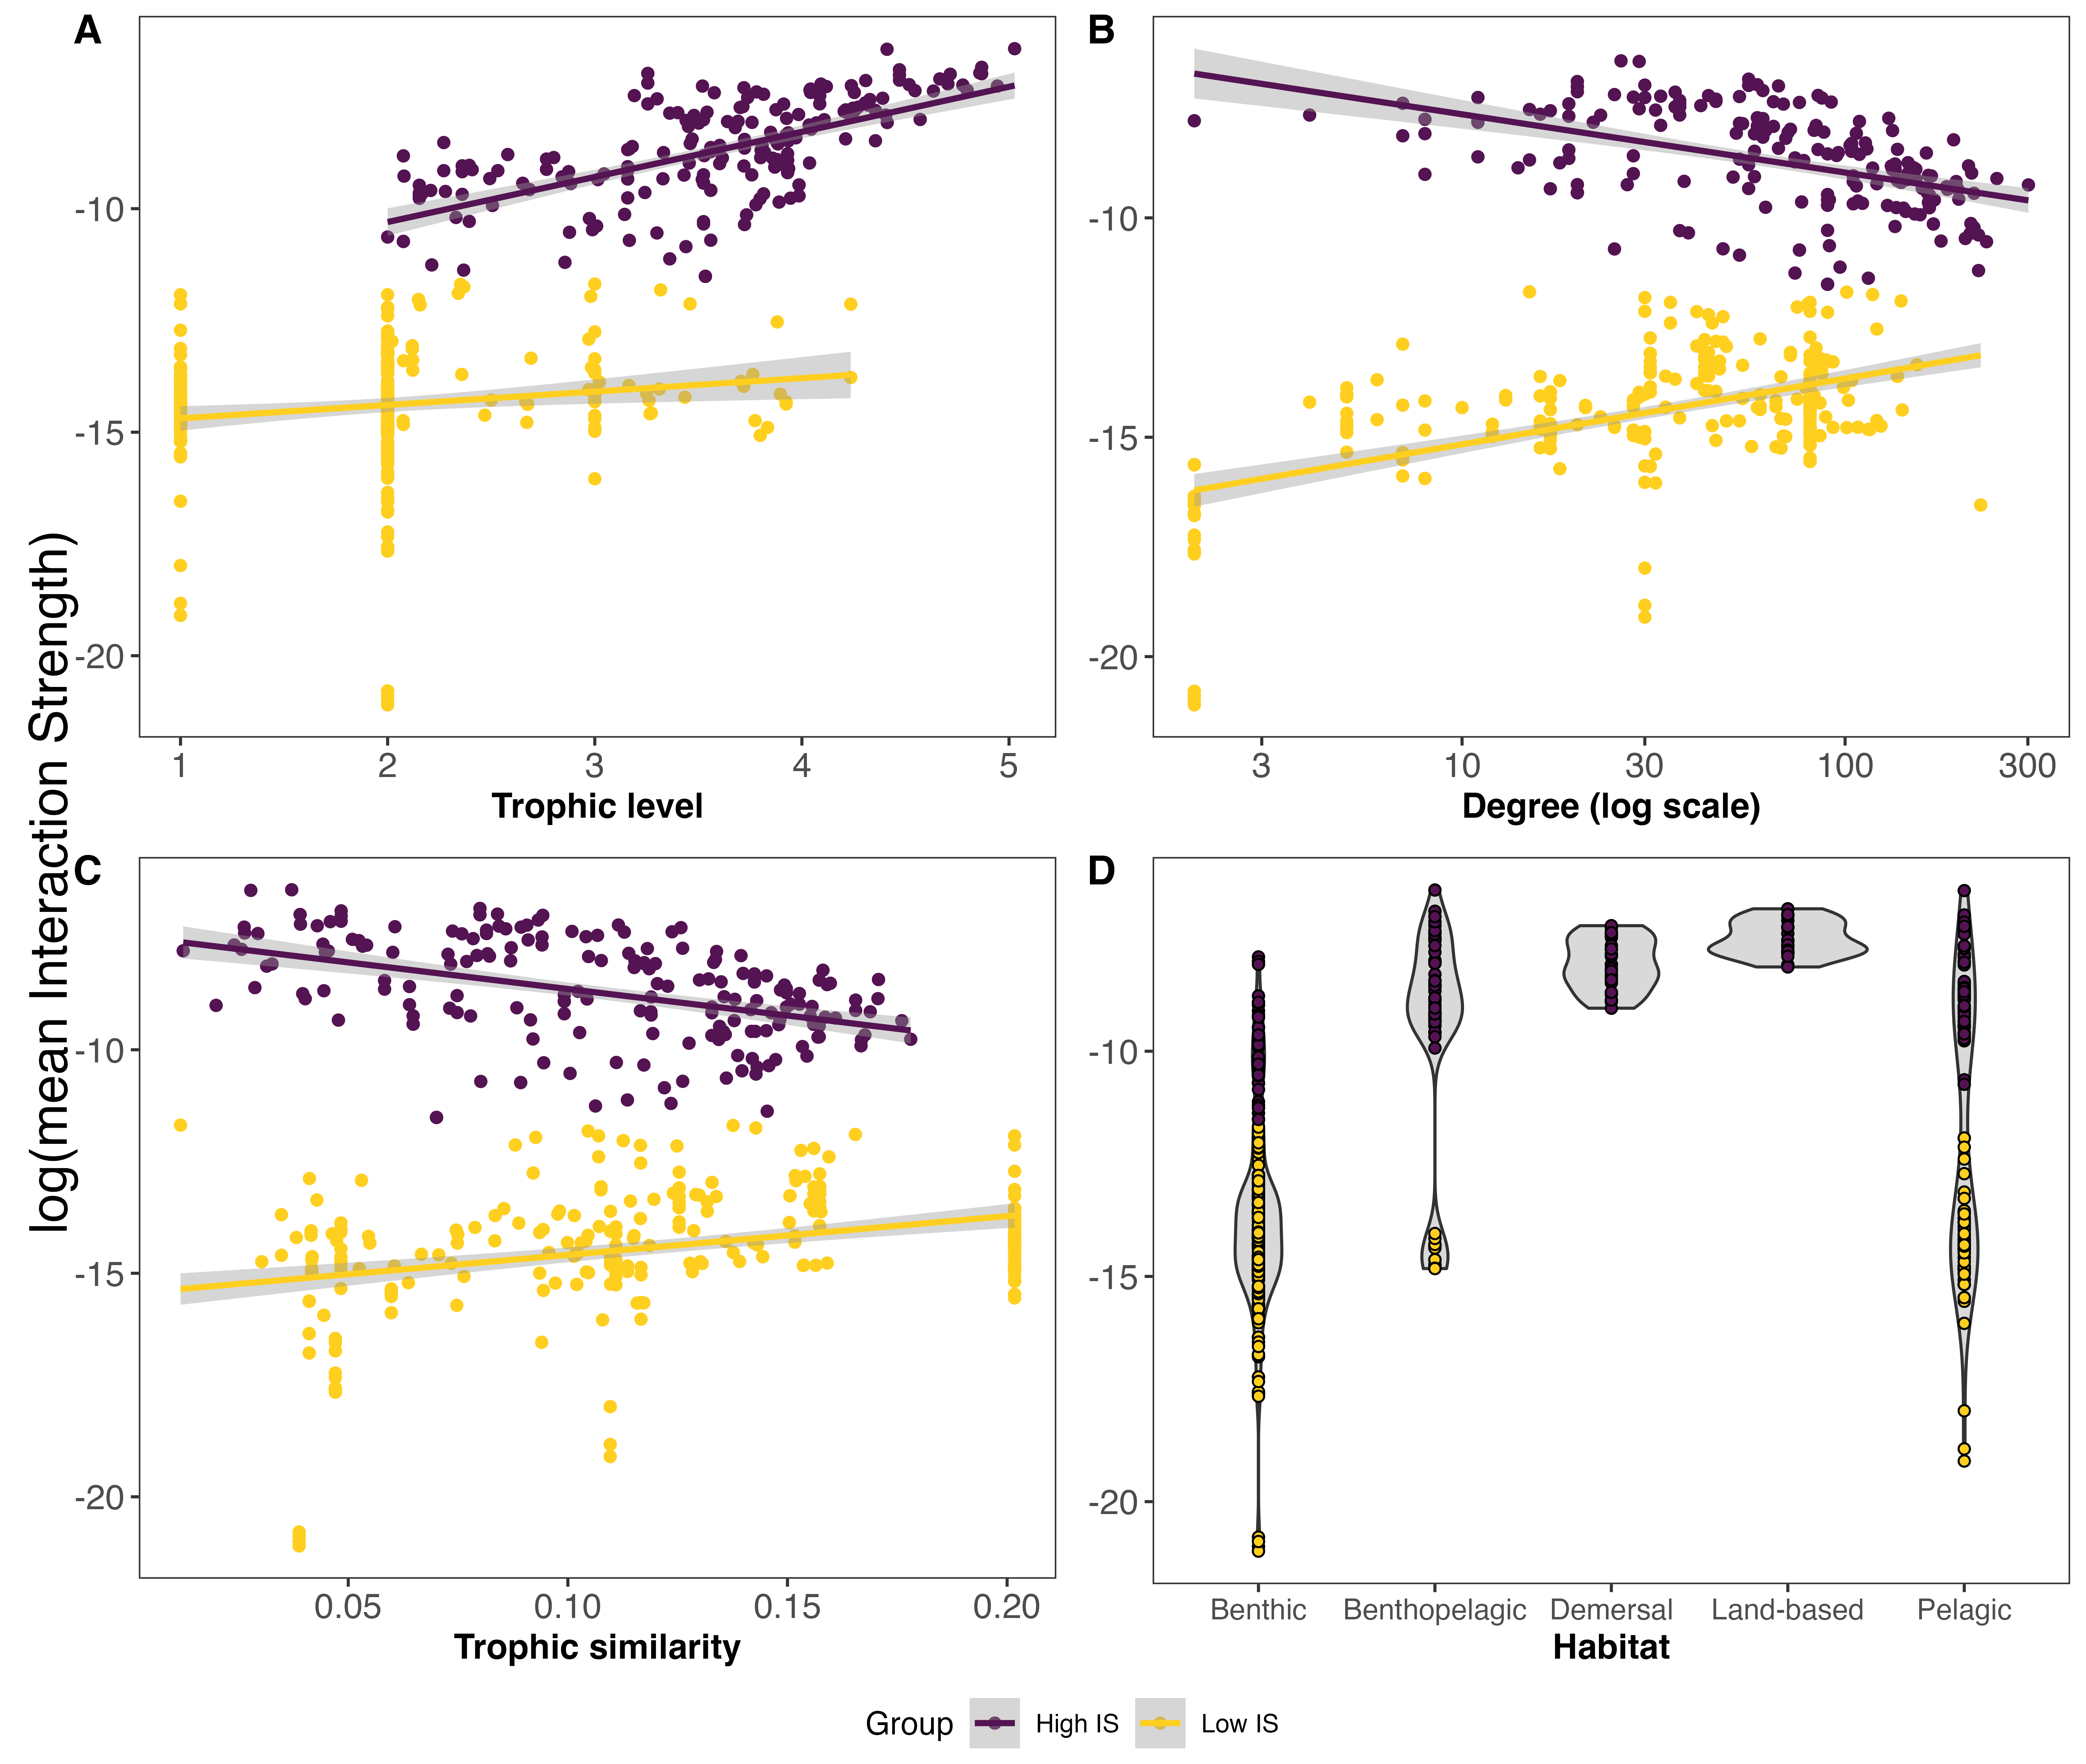
\includegraphics[width=12cm]{Fig4_LinReg} \caption{Relationships between weighted (mean Interaction Strength) and unweighted properties including habitat. Linear regressions are shown between log(mean interaction strength) and trophic level (A), degree (B) and trophic similarity (C). Linear regressions for trophic level ($y = 1.12x - 15.29, R^2 = 0.43, p-value < 2e-16$), degree ($y = 0.006x - 12.77, R^2 = 0.03, p-value = 4.06e-5$) and trophic similarity ($y = -1.46x - 12.18, R^2 = -0.0004, p-value = 0.36$).}\label{fig:unnamed-chunk-4}
\end{figure}

\clearpage

\begin{figure}
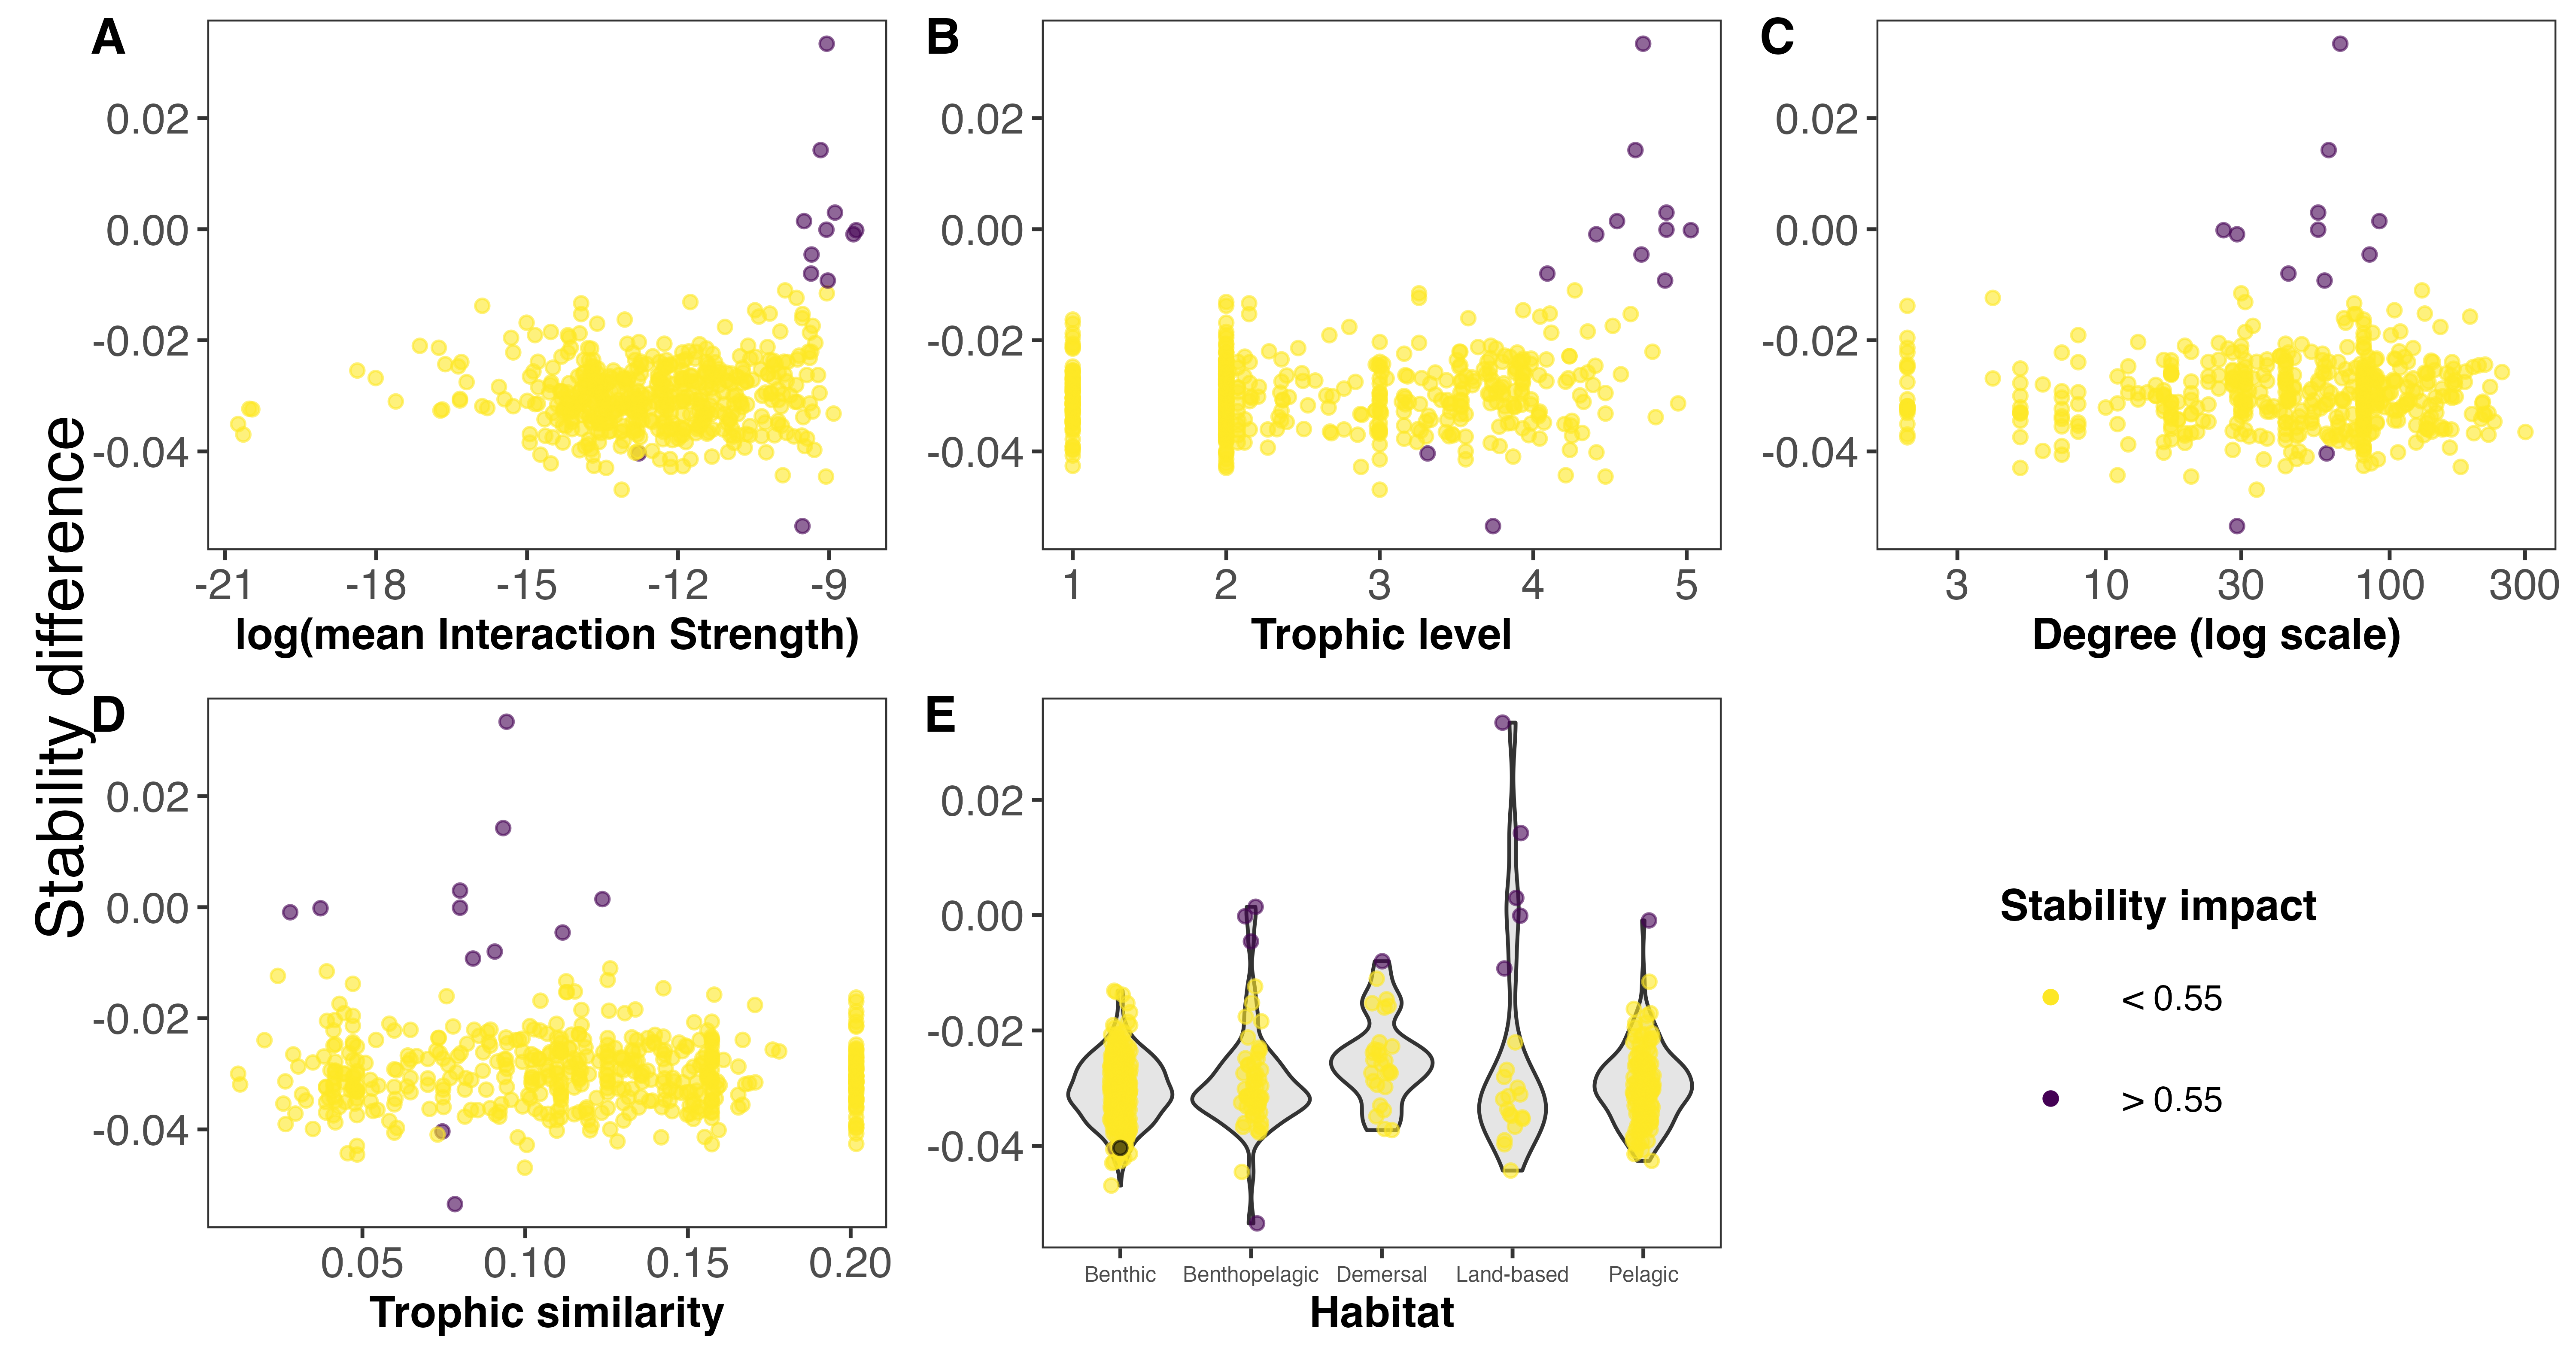
\includegraphics[width=12cm]{Fig.5_QSSDif} \caption{Stability  difference (mean maximum eingenvalue) between the whole Weddell Sea food web (n = 490) and the food web minus one species (n = 489) for weighted (interaction strength) and unweighted species properties, and habitat. Point color indicates the impact on the stability; if significant the extinction of that species altered the stability of the food web.}\label{fig:unnamed-chunk-5}
\end{figure}

\clearpage

\begin{table}[t]
\caption{Properties of the species that when become extinct generated a significant impact on the stability of the Weddell Sea food web, ordered by significance (Anderson-Darling p-value). References: meanIS = mean interaction strength, TL = trophic level, Deg = degree, TS = trophic similarity, StabDif = stability difference, ADvalue = Anderson-Darling p-value.}
\begin{tabular}{l c c c c c c c}
\tophline

\textbf{Species} & \textbf{meanIS} & \textbf{TL} & \textbf{Deg} & \textbf{TS} & \textbf{Habitat} & \textbf{StabDif} & \textbf{ADvalue}\\
\middlehline
Orcinus orca & 1.83e-4 & 5.03 & 26 & 0.037 & Benthopelagic & 4.67e-5 & 2.28e-41 \\
\middlehline
Macrourus holotrachys & 8.30e-5 & 4.70 & 85 & 0.112 & Benthopelagic & 3.55e-5 & 2.73e-23 \\
\middlehline
Pagetopsis macropterus & 7.08e-5 & 4.64 & 76 & 0.113 & Demersal & -1.80e-5 & 2.38e-12 \\
\middlehline
Abyssorchomene nodimanus & 2.56e-5 & 4.21 & 137 & 0.130 & Benthopelagic & 2.30e-5 & 8.52e-10 \\
\middlehline
Dissostichus mawsoni & 7.82e-5 & 4.12 & 87 & 0.126 & Pelagic & 2.17e-5 & 1.57e-9 \\
\middlehline
Macrourus whitsoni & 7.14e-5 & 4.55 & 92 & 0.124 & Benthopelagic & 2.12e-5 & 3.30e-8 \\
\middlehline
Hydrurga leptonyx & 1.03e-4 & 4.72 & 67 & 0.094 & Land-based & 2.04e-5 & 9.66e-6 \\
\middlehline
Mesonychoteuthis hamiltoni & 1.80e-4 & 4.41 & 29 & 0.028 & Pelagic & 1.82e-5 & 4.59e-5 \\
\middlehline
Champsocephalus gunnari & 7.62e-5 & 3.72 & 46 & 0.086 & Pelagic & 1.83e-5 & 6.79e-5 \\
\middlehline
Notothenia marmorata & 8.27e-5 & 4.09 & 44 & 0.091 & Demersal & 1.60e-5 & 1.23e-4 \\
\middlehline
Arctocephalus gazella & 9.28e-5 & 4.67 & 61 & 0.093 & Land-based & 1.17e-5 & 2.09e-4 \\
\middlehline
Trematomus pennellii & 3.04e-5 & 4.04 & 192 & 0.158 & Demersal & 1.44e-5 & 1.00e-3 \\
\middlehline
Mirounga leonina & 1.20e-4 & 4.87 & 56 & 0.080 & Land-based & 1.41e-5 & 1.28e-3 \\
\middlehline
Notothenia coriiceps & 4.94e-5 & 4.27 & 130 & 0.126 & Demersal & 1.44e-5 & 1.66e-3 \\
\middlehline
Maxilliphimedia longipes & 2.21e-6 & 3.26 & 60 & 0.136 & Benthopelagic & -4.46e-6 & 9.74e-3 \\

\bottomhline
\end{tabular}
\end{table}

\appendixfigures
\clearpage

\begin{figure}
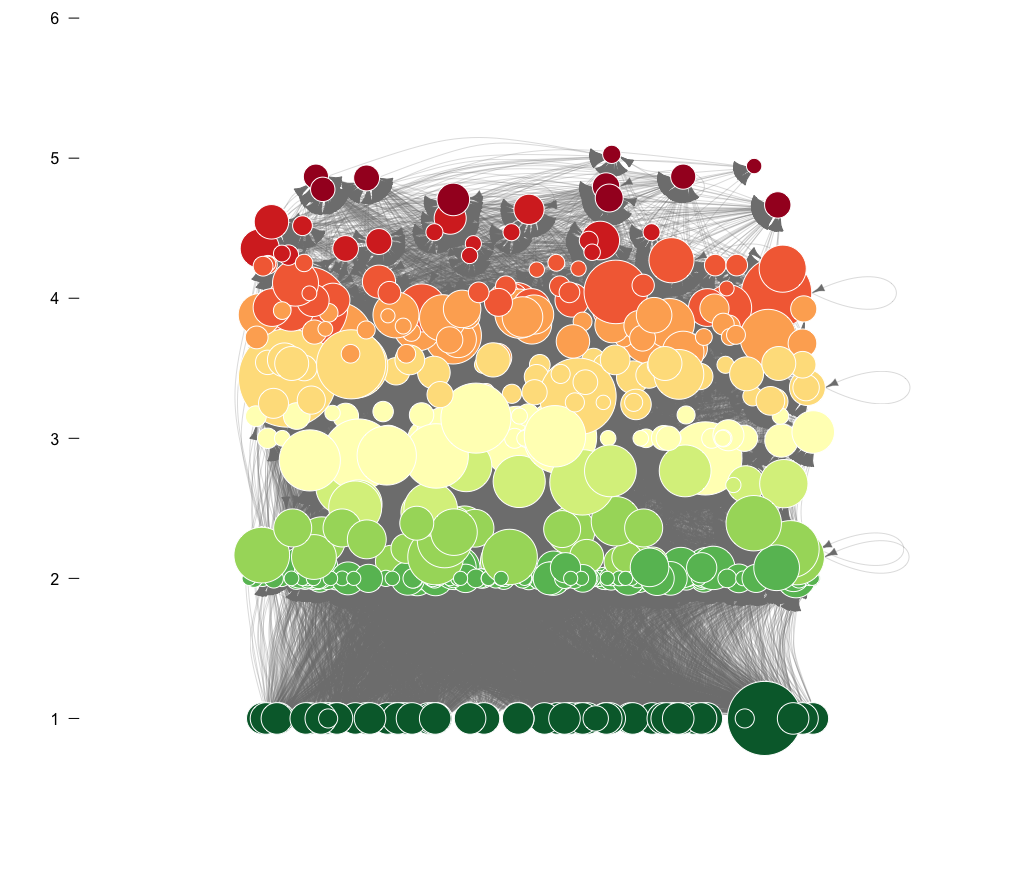
\includegraphics[width=12cm]{App1_FWplot} \caption{Graphic representation of the Weddell Sea food web. Species (nodes) are arranged vertically and colored by trophic level. The diameter of the node indicates the total number of interactions. Predator-prey interactions are represented by the arrows, from prey to predator.}\label{fig:unnamed-chunk-6}
\end{figure}






%%%%%%%%%%%%%%%%%%%%%%%%%%%%%%%%%%%%%%%%%%
%% optional

%%%%%%%%%%%%%%%%%%%%%%%%%%%%%%%%%%%%%%%%%%

%%%%%%%%%%%%%%%%%%%%%%%%%%%%%%%%%%%%%%%%%%
\authorcontribution{TIM and LAS: Conceptualization (lead); Data curation
(lead); Formal analysis (lead); Methodology (lead); Coding (lead);
Writing -- original draft (lead); Writing -- review and editing (lead).
SK: Conceptualization (lead); Formal analysis (supporting); Methodology
(supporting); Coding (supporting); Writing -- original draft
(supporting); Writing -- review and editing
(supporting).} %% optional section

%%%%%%%%%%%%%%%%%%%%%%%%%%%%%%%%%%%%%%%%%%
\competinginterests{The authors declare no competing
interests.} %% this section is mandatory even if you declare that no competing interests are present

%%%%%%%%%%%%%%%%%%%%%%%%%%%%%%%%%%%%%%%%%%

%%%%%%%%%%%%%%%%%%%%%%%%%%%%%%%%%%%%%%%%%%
\begin{acknowledgements}
Thanks to the rticles contributors!
\end{acknowledgements}

%% REFERENCES
%% DN: pre-configured to BibTeX for rticles

%% The reference list is compiled as follows:
%%
%% \begin{thebibliography}{}
%%
%% \bibitem[AUTHOR(YEAR)]{LABEL1}
%% REFERENCE 1
%%
%% \bibitem[AUTHOR(YEAR)]{LABEL2}
%% REFERENCE 2
%%
%% \end{thebibliography}

%% Since the Copernicus LaTeX package includes the BibTeX style file copernicus.bst,
%% authors experienced with BibTeX only have to include the following two lines:
%%
\bibliographystyle{copernicus}
\bibliography{../WeddellSea.bib}
%%
%% URLs and DOIs can be entered in your BibTeX file as:
%%
%% URL = {http://www.xyz.org/~jones/idx_g.htm}
%% DOI = {10.5194/xyz}


%% LITERATURE CITATIONS
%%
%% command                        & example result
%% \citet{jones90}|               & Jones et al. (1990)
%% \citep{jones90}|               & (Jones et al., 1990)
%% \citep{jones90,jones93}|       & (Jones et al., 1990, 1993)
%% \citep[p.~32]{jones90}|        & (Jones et al., 1990, p.~32)
%% \citep[e.g.,][]{jones90}|      & (e.g., Jones et al., 1990)
%% \citep[e.g.,][p.~32]{jones90}| & (e.g., Jones et al., 1990, p.~32)
%% \citeauthor{jones90}|          & Jones et al.
%% \citeyear{jones90}|            & 1990


\end{document}
